%!TEX root = Main.tex
\documentclass[Main]{subfiles}

\begin{document}
\section{Kalman} % (fold)
	\label{sec:kalman}
In this section the theory about basic Kalman Filter (KF) and the Extended Kalman Filter (EKF) will be introduced.
\subsection{The Kalman Filter}
The KF is a technique for filtering and predicting a linear system. 
It can be extended to also work on non-linear system, thus the EFK. 
The system in both KF and EKF is presented as a state-space model.
\autoref{eq:ss_state_eq1} and \autoref{eq:ss_state_eq2} shows the state-space model equations for the KF.
\begin{equation}
\label{eq:ss_state_eq1}
\mathbf{x}_k = \mathbf{A}_k \mathbf{x}_{k-1} + \mathbf{B}_k \mathbf{u}_k + \mathbf{w}_k
\end{equation}
\begin{equation}
\label{eq:ss_state_eq2}
\mathbf{z}_k = \mathbf{H}_k \mathbf{x}_k + \mathbf{v}_k
\end{equation}
In these equations $k$ is the time index, $\mathbf{x}_k$ and $\mathbf{x}_{k-1}$ is state vector at the different time instances, $\mathbf{u}_k$ is the control vector, $\mathbf{z}_k$ is the measurement vector, $\mathbf{A}_k$ is the state transition matrix of the system, $\mathbf{B}_k$ is the control matrix, $\mathbf{H}_k$ is the output measurement matrix, $\mathbf{w}_k$ is the process noise vector and $\mathbf{v}_k$ is the measurement noise vector.
The two noise vector are assumed to be Gaussian zero-mean white noise with the covariances $\mathbf{Q}$ and $\mathbf{R}$, where $\mathbf{Q}$ describes the covariance for the process noise and $\mathbf{R}$ for the measurement noise. 
It is also assumed that the noises are uncorrelated, \citep{Simon2006}.

The basic KF operates in a cyclic manner between two states; the time update state and the measurement update state, sometimes also called the prediction state and the correction state. 
This and the following description of the cyclic behavior, is based on \cite{Simon2006}.
The cyclic behavior is shown in \autoref{fig:cyclic_beha_kf}.
\begin{figure}[H]
	\centering
	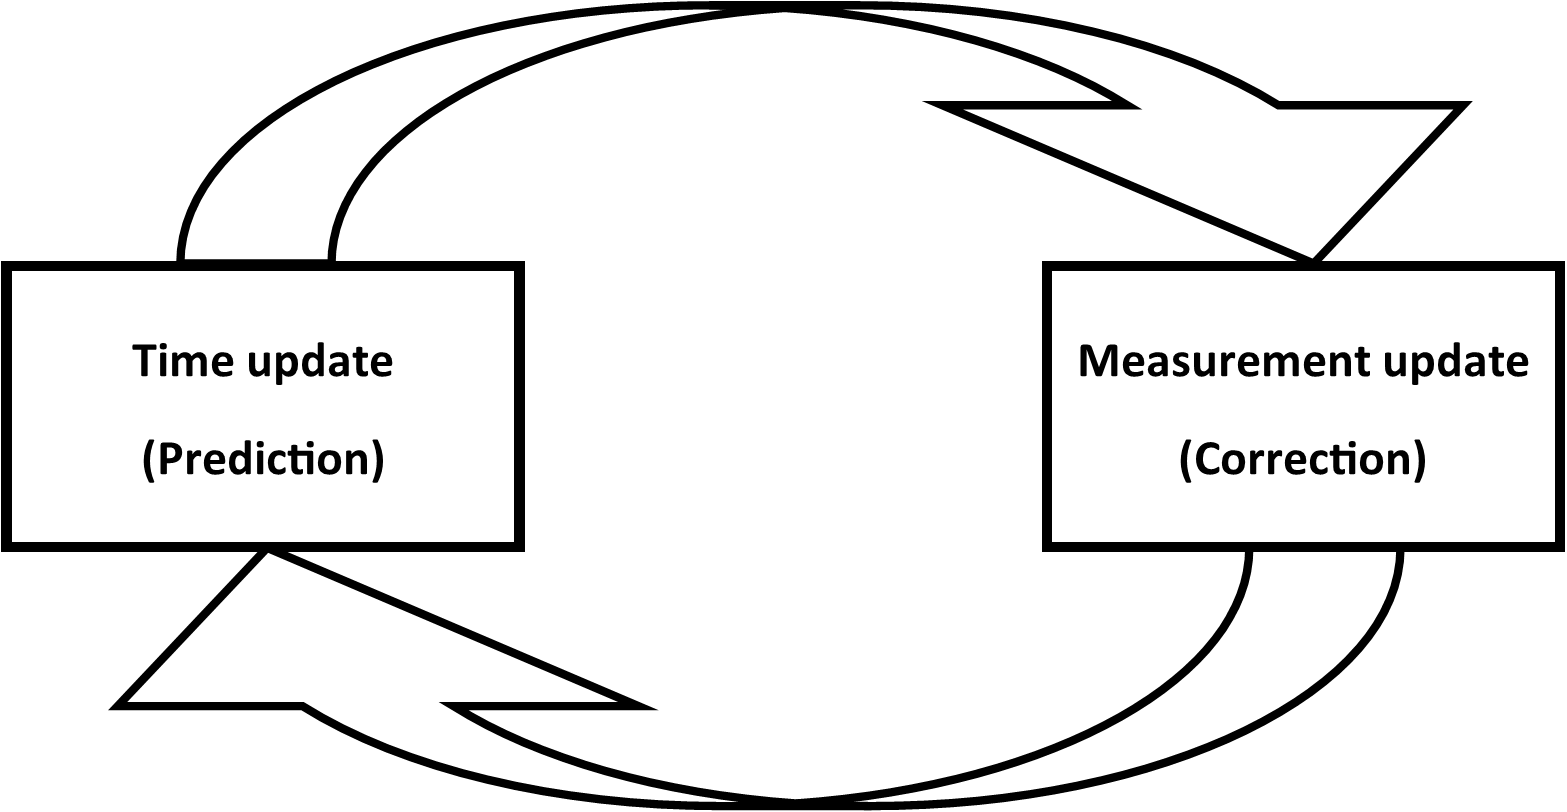
\includegraphics[width=0.5\linewidth]{./Figures/kf_states.png}
	\caption{The cyclic behavior of the KF}
	\label{fig:cyclic_beha_kf}
\end{figure}\noindent
Each of these states consists of several equations. The prediction state uses the state-space model to calculate a prediction of the state called the a priori state, \autoref{eq:kf_state_apriori}.
A priori is marked with a '$^-$'.
\begin{equation}
\label{eq:kf_state_apriori}
\mathbf{x}_k^-=\mathbf{A} \mathbf{x}_{k-1} + \mathbf{B} \mathbf{u}_k
\end{equation}
Here it is assumed that the system and control matrices are constant at all time instances.
It also predicts an a priori covariance of the state, that describes how certain the prediction is, \autoref{eq:kf_cov_apriori}.
\begin{equation}
\label{eq:kf_cov_apriori}
\mathbf{P}_k^-=\mathbf{A} \mathbf{P}_{k-1} \mathbf{A}^T+\mathbf{Q}
\end{equation}
The correction state then starts by calculating the Kalman Gain. 
The Kalman Gain is a matrix of weights, that show how much belief there is in the prediction and the measurement. \autoref{eq:kalman_gain} is the calculation of it.
\begin{equation}
\label{eq:kalman_gain}
\mathbf{K}_k = \mathbf{P}_k^- \mathbf{H}^T (\mathbf{H} \mathbf{P}_k^- \mathbf{H}^T + \mathbf{R})^{-1}
\end{equation}
The Kalman Gain is then used to correct the states as shown in \autoref{eq:kf_state_posterior}, thereby calculation what is called the posterior state. 
Posterior is marked with a '$^+$'.
\begin{equation}
\label{eq:kf_state_posterior}
\mathbf{x}_k^+ = \mathbf{x}_k^- + \mathbf{K}_k (\mathbf{z}_k - \mathbf{H} \mathbf{x}_k^-)
\end{equation}
The a priori covariance is also corrected to the posterior covariance by using the Kalman Gain, \autoref{eq:kf_cov_posterior}.
\begin{equation}
\label{eq:kf_cov_posterior}
\mathbf{P}_k^+ = (\mathbf{I} - \mathbf{K}_k \mathbf{H}) \mathbf{P}_k^-
\end{equation}
By looking at these equations, it can be seen that a KF actually describes how mean and covariance of the states propagates in time.
This becomes obvious when looking at an 1D example from \citep{Thrun2002}.

In this example a robot is moving in 1D.
\autoref{fig:kf_ex}a shows the a priori state and uncertainty, variance, of the robot.
This mean that the KF is in its prediction state.
The robot measures its position at \autoref{fig:kf_ex}b, and the uncertainty here is described by the measurement noise variance, $\mathbf{R}$.
The correction state calculates the Kalman Gain and finds the posterior state and uncertainty as seen in \autoref{fig:kf_ex}c.
Notice that the uncertainty now has a higher peak and smaller width.
The robot then moves in \autoref{fig:kf_ex}d, thereby adding uncertainty to its position.
This uncertainty is, as described in \autoref{eq:kf_cov_apriori}, the process noise variance, $\mathbf{Q}$; KF is back in the prediction state.
In \autoref{fig:kf_ex}e, it repeats the process from \autoref{fig:kf_ex}b.
And in \autoref{fig:kf_ex}f, it corrects itself like in \autoref{fig:kf_ex}c.
\begin{figure}[H]
	\centering
	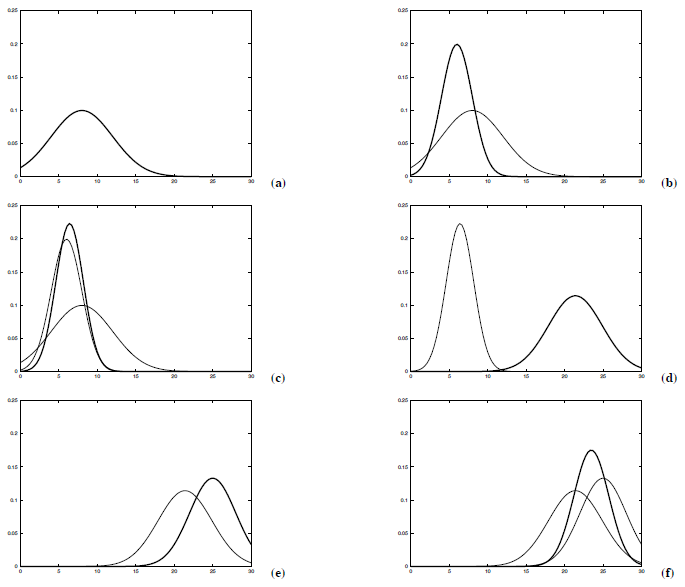
\includegraphics[width=0.8\linewidth]{./Figures/kf_ex.png}
	\caption{KF 1D example}
	\label{fig:kf_ex}
\end{figure}\noindent

\subsection{The Extended Kalman Filter}
	% section introduction (end)

\end{document}